% Capítulo resultante da fusão dos antigos capítulos "Integração do motor Prolog
% com o componente Java" e "Interface gráfica e arquitetura Web"; depois retiraram-se duas repetições.
% "do~sistema": o espaço inquebrável faz o título passar à linha depois de
% "arquitetura", com "do sistema" alinhado sob o texto do título.
\chapter{Notas adicionais sobre a arquitetura do~sistema}
\label{cap:arquitetura}

\section{Integração do motor Prolog com o componente Java}
\label{sec:integracao}

\cod{ExpertSystemBackend} define o ciclo comum aos motores: avançar o relógio,
iniciar o ciclo, inserir eventos, atualizar o veículo, decidir e expor a memória
e a explicação. \cod{PrologBackend} implementa esse contrato e permite trocar o
motor sem modificar o \cod{SimulationEngine}.

\paragraph{Comunicação.} O motor corre num processo \cod{swipl} persistente,
gerido pela classe \cod{PrologProcess}. O Java copia os ficheiros Prolog para
uma pasta de trabalho e arranca o processo com
\cod{swipl -q -g main -t halt server.pl}, que executa \cod{main/0} em \cod{server.pl}
e carrega os outros três ficheiros Prolog. Os dois lados trocam mensagens JSON
por \cod{stdin} e \cod{stdout}: um pedido por linha, e exatamente uma resposta
por linha, mesmo quando o pedido falhe. O processo é mantido vivo durante toda a
sessão: lançá-lo custa 150 a 250\,ms, incompatível com um ciclo de 100\,ms, e o
lado Prolog guarda estado entre ciclos. O \cod{server.pl} aceita quatro pedidos:
\cod{tick} (o ciclo de decisão), \cod{reset}, \cod{whynot} (\cref{sec:expl-whynot})
e \cod{dependencyIndex} (liga ou desliga o índice, só para o \emph{benchmark} da
\cref{sec:meta-indice}).

\paragraph{Pedidos e respostas.} Durante o ciclo, o \cod{PrologBackend} acumula
os eventos dos sensores. Preenche também um \cod{VehicleInput} com o estado do
veículo (velocidade, posição, via, manobra em curso, marcações e segurança das
vias adjacentes). Tudo segue num único pedido \cod{tick}, com
a decisão anterior (ação, regra e prioridade). A resposta traz as propostas
(ação, velocidade, risco, prioridade, razão, regra e evidência), os factos do
ciclo, o limite de velocidade em vigor, os subobjetivos da segurança de mudança de
via nos dois lados e as métricas do motor.

\paragraph{Arbitragem e aplicação.} O Java não decide nada por si: entrega as
propostas ao \cod{DecisionContext}. A
arbitragem trata em separado a velocidade e a via.

\begin{itemize}
  \item Na velocidade, as emergências e as paragens obrigatórias (prioridade 60
    ou mais) sobrepõem-se a tudo. Entre elas vence a mais prioritária e, em
    empate, a mais lenta. Abaixo disso, cada teto de velocidade que se verifica
    limita a velocidade de base, e decide o mais baixo, se ficar abaixo dessa
    base.
  \item Na via, vence a maior prioridade. Em empate, regressar à direita vence
    mudar de via.
  \item Uma mudança de via só é vetada quando uma paragem de prioridade
    superior está de facto a travar o veículo.
  \item Sem propostas, o veículo mantém a velocidade e a via.
\end{itemize}

O \cod{DecisionActuator} aplica a decisão ao veículo. Pode recusar uma mudança de
via que não consiga executar, e essa recusa fica registada. O ciclo, com o
resultado de cada proposta, é então guardado para o módulo de explicação
(\cref{sec:expl-registo}).

\section{Interface gráfica e arquitetura Web}
\label{sec:interface}

A aplicação segue uma arquitetura cliente-servidor.
O servidor, em Java~17 (ou superior) com Spring~Boot~3.3.4, corre a simulação e o motor de inferência.
O cliente é uma aplicação Angular~18 que só apresenta o estado e envia comandos.
A interface limita-se a desenhar o estado da simulação que o servidor envia:
nunca avalia condições de condução.

A comunicação usa dois canais: os comandos seguem por uma API REST, e o estado da
simulação chega por um WebSocket (\cod{/api/ws/simulation}), num \emph{snapshot}
em JSON a cada ciclo de 100\,ms.

A \emph{interface} (\cref{fig:interface-web}) mostra a estrada em perspetiva 3D, com o
veículo, os outros atores, a sinalização e a meteorologia.
Mostra também os painéis de explicação em tempo real (\cref{sec:expl-registo}) e
as leituras dos sensores.

Uma biblioteca de cenários e uma caixa de ferramentas permitem montar situações
durante a execução: veículos, peões, sinais, semáforos, buracos, obstáculos, barreiras e chuva.
Um seletor troca entre os motores Prolog e Drools, recarregando o cenário.

\begin{figure}[H]
  \centering
  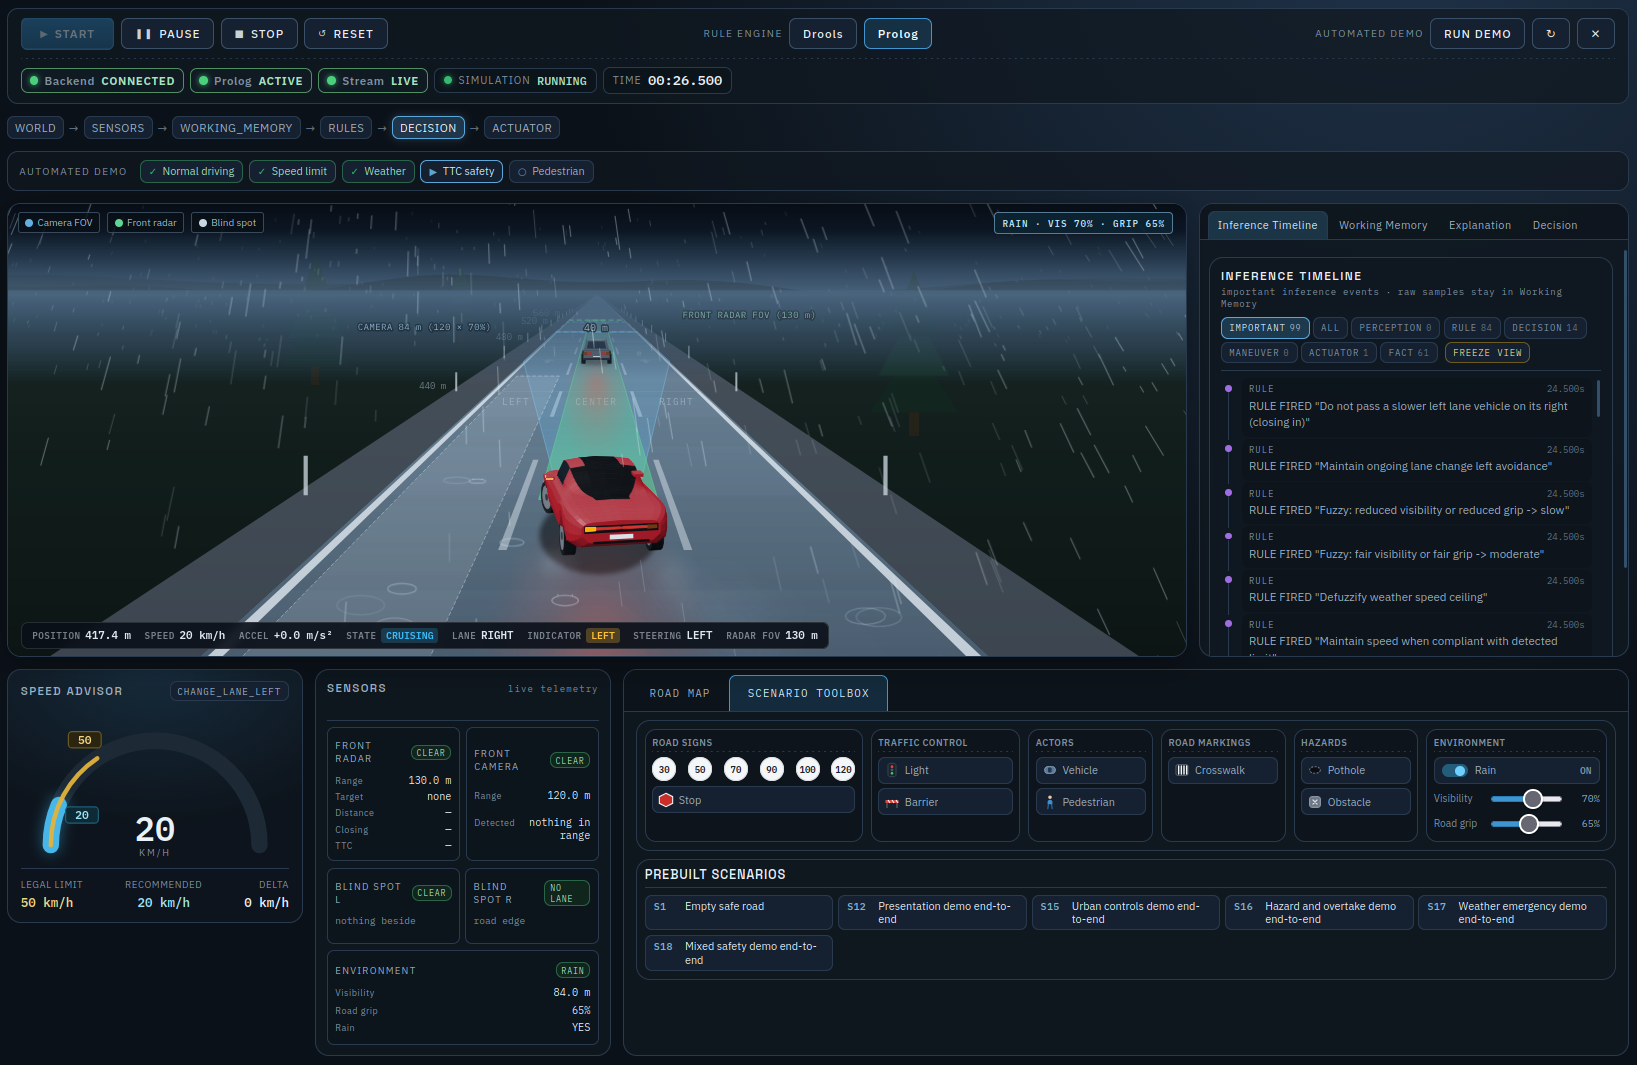
\includegraphics[width=0.72\textwidth]{figuras/screenshot-web-ui.png}
  \caption{Interface Web com o motor Prolog ativo, durante uma ultrapassagem com chuva.}
  \label{fig:interface-web}
\end{figure}
